\documentclass[11pt,a4paper]{article}

\usepackage[a4paper,landscape,margin=0.48in]{geometry}
\usepackage[T1]{fontenc}
\usepackage{lmodern}
\usepackage{microtype}
\usepackage{graphicx}
\usepackage{booktabs}
\usepackage{tabularx}
\usepackage{longtable}
\usepackage{array}
\usepackage{enumitem}
\usepackage{float}
\usepackage{xcolor}
\usepackage{hyperref}
\usepackage{xurl}

\definecolor{LineGray}{RGB}{95,101,107}
\definecolor{LightBlue}{RGB}{233,240,248}
\definecolor{LightYellow}{RGB}{250,244,225}
\definecolor{LightRed}{RGB}{249,232,230}
\definecolor{LinkBlue}{RGB}{35,82,124}

\hypersetup{
  colorlinks=true,
  linkcolor=LinkBlue,
  urlcolor=LinkBlue,
  pdftitle={How Algorithm 4 Ranks Equal-Edit-Distance Candidates}
}

\newcolumntype{Y}{>{\raggedright\arraybackslash}X}
\newcolumntype{L}[1]{>{\raggedright\arraybackslash}p{#1}}
\newcommand{\code}[1]{\texttt{#1}}
\newcommand{\good}{\textcolor{green!45!black}{better}}
\newcommand{\bad}{\textcolor{red!65!black}{worse}}
\graphicspath{{benchmark_04_experiments/results/04_meeting_10/figures/}{../results/04_meeting_10/figures/}}
\newcommand{\plot}[1]{%
  \includegraphics[width=0.96\linewidth,height=0.58\textheight,keepaspectratio]{#1}}

\setlength{\parindent}{0pt}
\setlength{\parskip}{0.30em}
\renewcommand{\arraystretch}{1.10}
\setlist[itemize]{leftmargin=1.35em,itemsep=0.12em,topsep=0.18em}
\setlist[enumerate]{leftmargin=1.55em,itemsep=0.12em,topsep=0.18em}
\clubpenalty=10000
\widowpenalty=10000
\displaywidowpenalty=10000

\begin{document}

\section{The Actual Deployed Order}

Algorithm 4 applies the following stages in this order. This is the operational
answer to ``what gets priority?''

\begin{table}[H]
\centering
\small
\begin{tabularx}{\linewidth}{@{}cL{0.18\linewidth}L{0.31\linewidth}Y@{}}
\toprule
\textbf{Stage} & \textbf{What happens} & \textbf{Exact rule} & \textbf{Example and consequence} \\
\midrule
1 & Normalize the query & Remove case, spaces, and punctuation for spelling comparison while retaining context separately. & \code{CLEX A NE} and \code{clexane} share compact form \code{clexane}. \\
2 & Retrieve candidates & Collect candidates from Algorithm 2, cleaned-context search, and Algorithm 4 rescue indexes. & A family found by two paths carries stronger independent support than a rescue-only family. \\
3 & Merge by family & Combine duplicate records that represent the same commercial family. & Strength or package variants do not receive several independent votes merely because the catalog contains several rows. \\
4 & Calculate evidence & Attach ordinary distance, weighted distance, position, edge, family, n-gram, skeleton, phonetic, and length evidence. & Two distance-1 candidates can receive different weighted, edge, and retriever-agreement values. \\
5 & Initial ranking & Sort by combined Algorithm 4 score, highest first. If scores are exactly equal, use the medicine name as a deterministic display fallback. & Equal ordinary distance alone does not change the existing score order. Alphabetic order is never treated as medical evidence. \\
6 & Bounded correction & Replace the first candidate only under a narrow rule listed in Table~\ref{tab:corrections}. Most rules require the alternative to be strictly closer. & A candidate at distance 1 can replace a distance-2 result when two retrievers support it and the score gap is small. \\
7 & Safety output & If the first two candidates have equal ordinary distance, label the response \code{equal\_distance\_ambiguity} and show alternatives. & The first item is display order, not a claim that the other option is medically impossible. \\
\bottomrule
\end{tabularx}
\caption{The deployed order. There is no universal ``first letter, then last letter, then alphabetic'' chain.}
\label{tab:actual-order}
\end{table}

\begin{center}
\fcolorbox{LineGray}{LightYellow}{%
\begin{minipage}{0.92\linewidth}
\textbf{What happens specifically when ordinary distances are equal?}
Stage 6 normally does nothing because its main corrections require a strictly
closer alternative. Stage 5 therefore decides the display order using the
combined score, and Stage 7 marks the answer ambiguous. The pure-deletion rule
is the bounded exception: a clean missing-letter relation may be promoted when
its score is close enough.
\end{minipage}}
\end{center}

\clearpage
\section{What The Combined Score Contains}


\setcounter{subsection}{1}
\setcounter{table}{3}
\subsection{Lexical Rescue Signals And Weights}



\small
\begin{longtable}{@{}L{0.19\linewidth}rL{0.30\linewidth}L{0.35\linewidth}@{}}
\caption{Every main signal in the Algorithm 4 rescue score.}\label{tab:lexical-signals}\\
\toprule
\textbf{Signal} & \textbf{Weight} & \textbf{Plain-English meaning} & \textbf{Example} \\
\midrule
\endfirsthead
\toprule
\textbf{Signal} & \textbf{Weight} & \textbf{Plain-English meaning} & \textbf{Example} \\
\midrule
\endhead
Exact family & 1.25 & Compact query exactly equals a catalog family. & \code{RIVOTRIL}$\rightarrow$\code{RIVOTRIL}. Exact evidence is strong, but an exact different real drug is treated as a collision in fair evaluation. \\
Ordinary edit similarity & 0.58 & Rewards fewer ordinary edits after accounting for string length. & Both \code{CEFAXIM} and \code{CEFIXIME} are one ordinary edit from \code{CEFAXIME}, so this signal ties. \\
Weighted edit similarity & 0.52 & Gives lower cost to known confusion pairs and vowel changes. Known pairs cost 0.45, vowel-to-vowel changes cost 0.70, and an ordinary replacement costs 1. & For \code{CEFAXIME}, \code{CEFIXIME} has weighted distance 0.70 while \code{CEFAXIM} has 1.00. Weighted spelling therefore favors \code{CEFIXIME}. \\
Same-position evidence & 0.24 & Measures how many query characters remain in the same index positions. & \code{CEFAXIME} and \code{CEFIXIME} match in seven of eight positions, producing 0.875. \\
Character 3-grams & 0.18 & Compares overlapping three-character pieces. & \code{RIVOTIL} and \code{RIVOTRIL} share pieces such as \code{RIV}, \code{IVO}, and \code{VOT}. \\
Prefix evidence & 0.16 & Measures the uninterrupted matching characters from the beginning. & \code{CLARANE} and \code{CLARA} share the beginning \code{CLARA}; this can be useful but can also favor a shorter wrong family. \\
Consonant skeleton & 0.16 & Compares a reduced spelling key that preserves consonant structure. & \code{NOW} and \code{NEW} both preserve the frame \code{NW}. The signal therefore recognizes their shared frame but cannot decide which full name was seen. \\
Length coverage & 0.16 & Rewards candidates whose length is close to the query length. & For query \code{CEFAXIME}, eight-character \code{CEFIXIME} has full length coverage, while seven-character \code{CEFAXIM} has coverage $7/8=0.875$. \\
Phonetic key & 0.14 & Compares normalized sound-confusion groups such as C/K/Q, F/V, P/B, D/T, and S/Z. & \code{COUFSED} can retain phonetic evidence for \code{COUGHSED}; phonetic agreement still needs spelling or retrieval support. \\
Suffix evidence & 0.10 & Measures uninterrupted matching characters from the end. & \code{ANYOLAX} and \code{MYOLAX} share the ending \code{YOLAX}. \\
Character 2-grams & 0.10 & Compares overlapping two-character pieces. & \code{MYMLAX} and \code{MYOLAX} retain several neighboring letter pairs despite one OCR replacement. \\
Ordered subsequence & 0.10 & Rewards query letters that appear in the candidate in the same order even when characters are missing between them. & \code{RIVOTRI} is an ordered subsequence of \code{RIVOTRIL}. \\
\bottomrule
\end{longtable}
\normalsize

\subsection{Bonuses And Penalties}

\begin{table}[H]
\centering
\small
\begin{tabularx}{\linewidth}{@{}L{0.22\linewidth}rL{0.30\linewidth}Y@{}}
\toprule
\textbf{Condition} & \textbf{Change} & \textbf{Meaning} & \textbf{Specific word example} \\
\midrule
Same first character & $+0.12$ & Useful evidence, but too small to become a universal first-character rule. & Query \code{CEFAXIME} and candidate \code{CEFIXIME} both start with C, so this candidate receives $+0.12$. \\
Confusable first characters & $+0.06$ & Keeps a candidate when the first letters belong to a known confusion group such as P/B or C/K. & Illustrative query \code{BANDOL} and candidate \code{PANDOL} start with confusable B/P, so the candidate receives $+0.06$, not the full same-letter bonus. \\
Length difference at most 1 and weighted similarity at least 0.76 & $+0.18$ & Rewards a compact near-match only when its spelling is already strong. & \code{CEFAXIME}$\rightarrow$\code{CEFIXIME} has equal length and weighted similarity $1-0.70/8=0.9125$, so it receives $+0.18$. \\
Prefix at least 0.55 and weighted similarity at least 0.66 & $+0.08$ & Rewards a strong beginning only when the complete spelling is also plausible. & \code{CLARANE}$\rightarrow$\code{CLARA} shares five starting characters, prefix $5/7=0.714$, and remains close enough to receive the bonus. \\
Weighted similarity at least 0.84 and position at least 0.70 & $+0.22$ & Rewards agreement between two independent spelling measurements. & \code{CEFAXIME}$\rightarrow$\code{CEFIXIME} has weighted similarity 0.9125 and position evidence 0.875, so both conditions pass. \\
Short partial prefix with weak weighted evidence & $-0.18$ to $-0.42$ & Stops a short prefix from beating a stronger complete-name candidate merely because its beginning matches. & \code{ABIMOL}$\rightarrow$\code{ABIMOL EXTRA} is a clean prefix but covers only part of the longer family, so weak full-name evidence can trigger the maximum $-0.42$ penalty. \\
Very short non-exact query with weak edit evidence & $-0.22$ & Reduces confident matches from three- or four-character noise. & \code{ABC}$\rightarrow$\code{ABC IMMUNE} shares a prefix, but the three-character non-exact query carries too little full-name evidence. \\
Weak spelling plus weak skeleton/phonetic evidence & $-0.20$ & Rejects candidates supported by no strong spelling or sound channel. & \code{GHONT}$\rightarrow$\code{CALAMINE} has severe spelling corruption and no strong skeleton or phonetic support, so this penalty applies. \\
Weak prefix, weak 3-grams, and weak edit evidence & $-0.10$ & Penalizes a candidate with little shared local structure. & \code{GHONT}$\rightarrow$\code{CALAMINE} also lacks a useful prefix and shared three-character pieces, so it can receive this additional penalty. \\
\bottomrule
\end{tabularx}
\caption{Bonuses require supporting conditions. No single bonus is an automatic winner.}
\label{tab:bonuses}
\end{table}

\section{The Bounded Corrections}

After sorting by combined score, Algorithm 4 permits only the following
evidence-backed changes to the first candidate. A score gap is the current
first candidate's score minus the alternative's score. The maximum gap prevents
a single spelling clue from overturning a much stronger multi-signal result.

\begin{table}[H]
\centering
\small
\begin{tabularx}{\linewidth}{@{}L{0.16\linewidth}L{0.29\linewidth}L{0.23\linewidth}Y@{}}
\toprule
\textbf{Correction} & \textbf{Required evidence} & \textbf{Why every condition is required} & \textbf{Specific word example} \\
\midrule
Strictly closer candidate & Both retrieval layers found the alternative; its ordinary distance is at most 2; it is at least one edit closer than the current first candidate; score gap is at most 0.25. & Agreement reduces the chance that one retrieval path produced noise. The distance and score-gap limits restrict the change to a small inversion, not a global edit-distance sort. & For \code{MYCLAX}, the baseline put \code{MICLOX} first and \code{MYOLAX} second. Both retrieval layers supported \code{MYOLAX}, which was one edit closer, so the correction moved \code{MYOLAX} to rank 1. \\
Pure deletion candidate & Query length is at least 5; it is an ordered subsequence of the candidate; exactly one or two missing characters explain the difference; candidate is no farther than the current first result; score gap is at most 0.40. & Every visible character must remain in order, so the rule models omitted unreadable letters rather than arbitrary similarity. This is the only correction that may act when ordinary distances are equal. & \code{RIVOTRI}$\rightarrow$\code{RIVOTRIL}: the query contains every candidate character except the final L, in the same order. It is eligible only if the competing result is no closer and the score gap stays within 0.40. \\
Single-token correction & Current first result contains several words; alternative contains one word; alternative is strictly closer with distance at most 2; score gap is at most 0.20. & The strict distance and small gap prevent a short medicine from replacing a valid multi-word family solely because it is shorter. & Query \code{ABIMOL} can retrieve multi-word \code{ABIMOL EXTRA} and single-family \code{ABIMOL}. The single exact family may move first only when the multi-word result initially leads by no more than 0.20. \\
Family-head correction & Catalog confirms a variant family; query has at least 5 characters; family head is within two edits and strictly closer than the current first family; score gap is at most 1.40. & Package text can make a full variant look far away even when its shared family head is close. Catalog-derived grouping is required so arbitrary prefixes cannot claim family membership. & \code{LANTS} originally placed the \code{LANTUS ...} variants at rank 15. The validated head \code{LANTUS} is one edit away, so the family-head correction moved those variants to rank 1 before variant selection. \\
Strict full-name correction & Query has at least 5 characters; rescue-only full name is within three edits and strictly closer; weighted distance is no worse; score gap is at most 0.35; current first result has no protected exact, prefix, or combined phonetic evidence. & The alternative must win on both ordinary and weighted spelling while staying close in total score. Protected evidence blocks the correction when the current result has a separate strong explanation. & \code{MYOLANA} originally placed \code{MYOLAX} second. The rescue full name was one edit closer within the 0.35 gap, so the correction moved \code{MYOLAX} to rank 1. \\
\bottomrule
\end{tabularx}
\caption{Except for the controlled pure-deletion relation, equal ordinary distance does not activate these corrections.}
\label{tab:corrections}
\end{table}

\section{Real Equal-Distance Examples}


\subsection{Worked Example: \code{CEFAXIME}}

\begin{table}[H]
\centering
\small
\begin{tabularx}{\linewidth}{@{}lrrY@{}}
\toprule
\textbf{Evidence} & \textbf{CEFAXIM} & \textbf{CEFIXIME} & \textbf{Interpretation} \\
\midrule
Ordinary edit distance & 1.00 & 1.00 & Tie. Ordinary edit distance cannot decide. \\
Weighted edit distance & 1.00 & \textbf{0.70} & \code{CEFIXIME} wins because A$\rightarrow$I is a vowel substitution. Lower is better. \\
Same-position evidence & 0.875 & 0.875 & Tie. Both preserve seven of eight positions. \\
Edge evidence & \textbf{0.875} & 0.500 & \code{CEFAXIM} wins because it matches the long beginning. \\
Dual-retriever agreement & yes & yes & Tie. Both retrieval layers found both families. \\
Combined score & \textbf{2.7582} & 2.5376 & Current order puts \code{CEFAXIM} first. \\
\bottomrule
\end{tabularx}
\caption{The signals genuinely disagree. Weighted spelling selects the verified family, while edge and full score select the other candidate. The correct product behavior is to show both and request confirmation.}
\label{tab:cefaxime}
\end{table}

\subsection{More Cases Showing Why One Rule Is Not Enough}

\begin{longtable}{@{}L{0.105\linewidth}L{0.115\linewidth}L{0.125\linewidth}L{0.215\linewidth}L{0.26\linewidth}@{}}
\caption{Real cases in which equal ordinary distance leaves conflicting evidence.}\label{tab:real-ties}\\
\toprule
\textbf{Input} & \textbf{Verified} & \textbf{Current first} & \textbf{Important values} & \textbf{Plain-English conclusion} \\
\midrule
\endfirsthead
\toprule
\textbf{Input} & \textbf{Verified} & \textbf{Current first} & \textbf{Important values} & \textbf{Plain-English conclusion} \\
\midrule
\endhead
\code{ANYOLAX} & \code{MYOLAX} & \code{AGIOLAX} & Both raw 2 and weighted 1.45. Position: 0.714 vs 0.000. Edge: 0.571 vs 0.714. Agreement: no vs yes. & Position-first keeps \code{AGIOLAX}; edge-first selects \code{MYOLAX}. The signals point in opposite directions. \\
\code{RIVOFN2} & \code{RIVOTRIL} & \code{RIOPAN} & Both raw 4 and weighted 4. Position: 0.429 vs 0.500. Edge: 0.286 vs 0.500. & Position-first and edge-first select \code{RIVOTRIL}. Weighted-first selects a third family, \code{REVAN}. Severe corruption creates several equally weak candidates. \\
\code{LAMIX} & \code{LASIX} & \code{VAMIX} & Both raw 1, weighted 1, and position 0.800. Edge: 0.800 vs 0.400. & Every tested generic rule retains \code{VAMIX}. Available evidence itself favors the wrong candidate, so changing tie order cannot solve the row. \\
\code{CLARANE} & \code{CLEXANE} & \code{CLARA} & Both raw 2. Weighted: 2.0 vs 1.7. Position ties at 0.714. Edge: 0.714 vs 0.429. & Weighted-first selects \code{CLEXANE}; edge-first keeps \code{CLARA}. A long shared prefix can conflict with better weighted spelling. \\
\code{INDEVIO} & \code{INDERAL} & \code{ENTYVIO} & Both raw 3. Weighted: 1.35 vs 2.70. Position ties at 0.571. Edge: 0.429 vs 0.571. Agreement: yes vs no. & Every tested rule retains \code{ENTYVIO}. The verified family does not dominate on the recorded evidence. \\
\code{CONAL} & \code{COBAL} & \code{CONIL} & Both candidates are one ordinary edit away and both share the same first character. & A first-character rule cannot break this tie. The safe response is candidate comparison. \\
\bottomrule
\end{longtable}

\section{The Eight Tie Orders That Were Tested}

\begin{longtable}{@{}L{0.20\linewidth}L{0.34\linewidth}rrr@{}}
\caption{Exact policy order and measured Hit@1. Higher is better.}\label{tab:policies}\\
\toprule
\textbf{Policy} & \textbf{Order used inside an eligible tie} & \textbf{All} & \textbf{Dev.} & \textbf{Holdout} \\
\midrule
\endfirsthead
\toprule
\textbf{Policy} & \textbf{Order used inside an eligible tie} & \textbf{All} & \textbf{Dev.} & \textbf{Holdout} \\
\midrule
\endhead
Current deployed order & Keep full Algorithm 4 score order. & \textbf{47.63\%} & 47.98\% & \textbf{46.24\%} \\
Weighted then position & Lower weighted cost; higher position; higher edge; agreement; full score. & 45.91\% & 46.36\% & 44.09\% \\
Position then weighted & Higher position; lower weighted cost; higher edge; agreement; full score. & 46.55\% & 46.63\% & \textbf{46.24\%} \\
Edge then weighted & Higher prefix/suffix edge; lower weighted cost; higher position; agreement; full score. & 47.41\% & \textbf{48.52\%} & 43.01\% \\
Composite evidence & Maximize $-d_w+0.35p+0.25e+0.10a$; then full score. & 46.12\% & 46.63\% & 44.09\% \\
Pareto, gap 0.25 & Switch only if no worse on weighted, position, edge, and agreement; better on at least one; score gap at most 0.25. & 46.77\% & 47.44\% & 44.09\% \\
Pareto, gap 0.15 & Same rule with score gap at most 0.15. & 46.77\% & 47.44\% & 44.09\% \\
Pareto, gap 0.10 & Same rule with score gap at most 0.10. & 46.55\% & 47.17\% & 44.09\% \\
\bottomrule
\end{longtable}


\clearpage
\section{Measured Importance of Algorithm 4 Components}

Every row below runs the same 464 fair, unique OCR query-target pairs. ``Without
X'' means that only component X was disabled. A negative delta means accuracy
fell after removing the component; a positive delta means the ablation scored
slightly higher on this sample.

\setcounter{table}{10}
\footnotesize
\begin{longtable}{@{}lrrrr@{}}
\caption{Complete 24-configuration ablation result on 464 primary pairs. Deltas
are percentage points relative to complete Algorithm 4.}\\
\toprule
\textbf{Configuration} & \textbf{Hit@1} & \textbf{Hit@20} &
\textbf{$\Delta$ H@1} & \textbf{$\Delta$ H@20} \\
\midrule
\endfirsthead
\toprule
\textbf{Configuration} & \textbf{Hit@1} & \textbf{Hit@20} &
\textbf{$\Delta$ H@1} & \textbf{$\Delta$ H@20} \\
\midrule
\endhead
Complete Algorithm 4 & 47.63\% & 71.12\% & 0.00 & 0.00 \\
Without external retriever & 47.20\% & 71.55\% & -0.43 & +0.43 \\
Without context cleanup & 47.63\% & 71.34\% & 0.00 & +0.22 \\
Without family rescue & 27.37\% & 51.08\% & -20.26 & -20.04 \\
Without raw edit similarity & 46.77\% & 65.30\% & -0.86 & -5.82 \\
Without weighted edit similarity & 46.34\% & 63.79\% & -1.29 & -7.33 \\
Without prefix evidence & 46.55\% & 68.53\% & -1.08 & -2.59 \\
Without suffix evidence & 47.63\% & 71.12\% & 0.00 & 0.00 \\
Without character n-grams & 46.77\% & 70.69\% & -0.86 & -0.43 \\
Without phonetic evidence & 47.20\% & 71.12\% & -0.43 & 0.00 \\
Without consonant skeleton & 46.98\% & 70.69\% & -0.65 & -0.43 \\
Without subsequence evidence & 47.20\% & 70.91\% & -0.43 & -0.22 \\
Without position evidence & 46.12\% & 69.40\% & -1.51 & -1.72 \\
Without length coverage & 47.20\% & 67.67\% & -0.43 & -3.45 \\
Without delete-key retrieval & 47.63\% & 70.91\% & 0.00 & -0.22 \\
Without short-edge retrieval & 46.77\% & 67.46\% & -0.86 & -3.66 \\
Without first-character expansion & 47.63\% & 71.12\% & 0.00 & 0.00 \\
Without compatible-length scan & 46.98\% & 68.97\% & -0.65 & -2.16 \\
Without family-head rescue & 44.61\% & 69.61\% & -3.02 & -1.51 \\
Without weighted confusion costs & 46.77\% & 70.69\% & -0.86 & -0.43 \\
Without retriever agreement & 47.20\% & 70.91\% & -0.43 & -0.22 \\
Without strict full-name correction & 46.55\% & 71.12\% & -1.08 & 0.00 \\
Without conservative reranker & 41.16\% & 70.47\% & -6.47 & -0.65 \\
Without safety clarification gate & 47.63\% & 71.12\% & 0.00 & 0.00 \\
\bottomrule
\end{longtable}
\normalsize

\textbf{Table 11 insights}
\begin{enumerate}
  \item Family rescue is the largest retrieval component: removing it loses
        20.26 Hit@1 points and 20.04 Hit@20 points.
  \item Weighted and raw edit similarity are complementary. Removing weighted
        similarity loses 7.33 Hit@20 points; removing raw similarity loses 5.82.
  \item The conservative reranker mainly changes order. Its removal loses 6.47
        Hit@1 points but only 0.65 Hit@20 points.
  \item The safety gate has zero retrieval delta because it changes confidence,
        not candidate rank. Removing it raises unsafe confident answers, which
        Hit@1 and Hit@20 cannot measure.
\end{enumerate}

\clearpage
\section{The Extreme-Distance Cohort Above 60\%}

\begin{minipage}[t]{0.49\linewidth}
\textbf{What ``extreme'' means.}
Let $q_c$ and $y_c$ be the OCR query and verified target after lowercasing and
removing spaces and punctuation. With Levenshtein distance $L$,
\[
  r=\frac{L(q_c,y_c)}{\max(|y_c|,1)},
  \qquad r>0.60\ \mathrm{means\ extreme}.
\]
This is an edit ratio, not confidence. For \code{PNO}$\rightarrow$\code{RIVO},
$L=3$, $|y_c|=4$, and $r=3/4=0.75$, so the row is extreme.
\end{minipage}
\hfill
\begin{minipage}[t]{0.48\linewidth}
\textbf{What a bigram means.}
A bigram is one adjacent two-character piece after the same compacting step.
\code{RIV} has \code{RI} and \code{IV}. \code{RIVOTRIL} has \code{RI},
\code{IV}, \code{VO}, \code{OT}, \code{TR}, \code{RI}, and \code{IL}.
The pair therefore retains two shared bigrams, \code{RI} and \code{IV}.
Shared bigrams measure preserved local letter order, not pronunciation.

\textbf{Denominator.}
The cohort has 121 of 595 observations (20.34\%) and 113 unique compact
query-target pairs; eight rows repeat a pair produced by another OCR model.
\end{minipage}

\setcounter{figure}{5}
\begin{figure}[H]
\centering
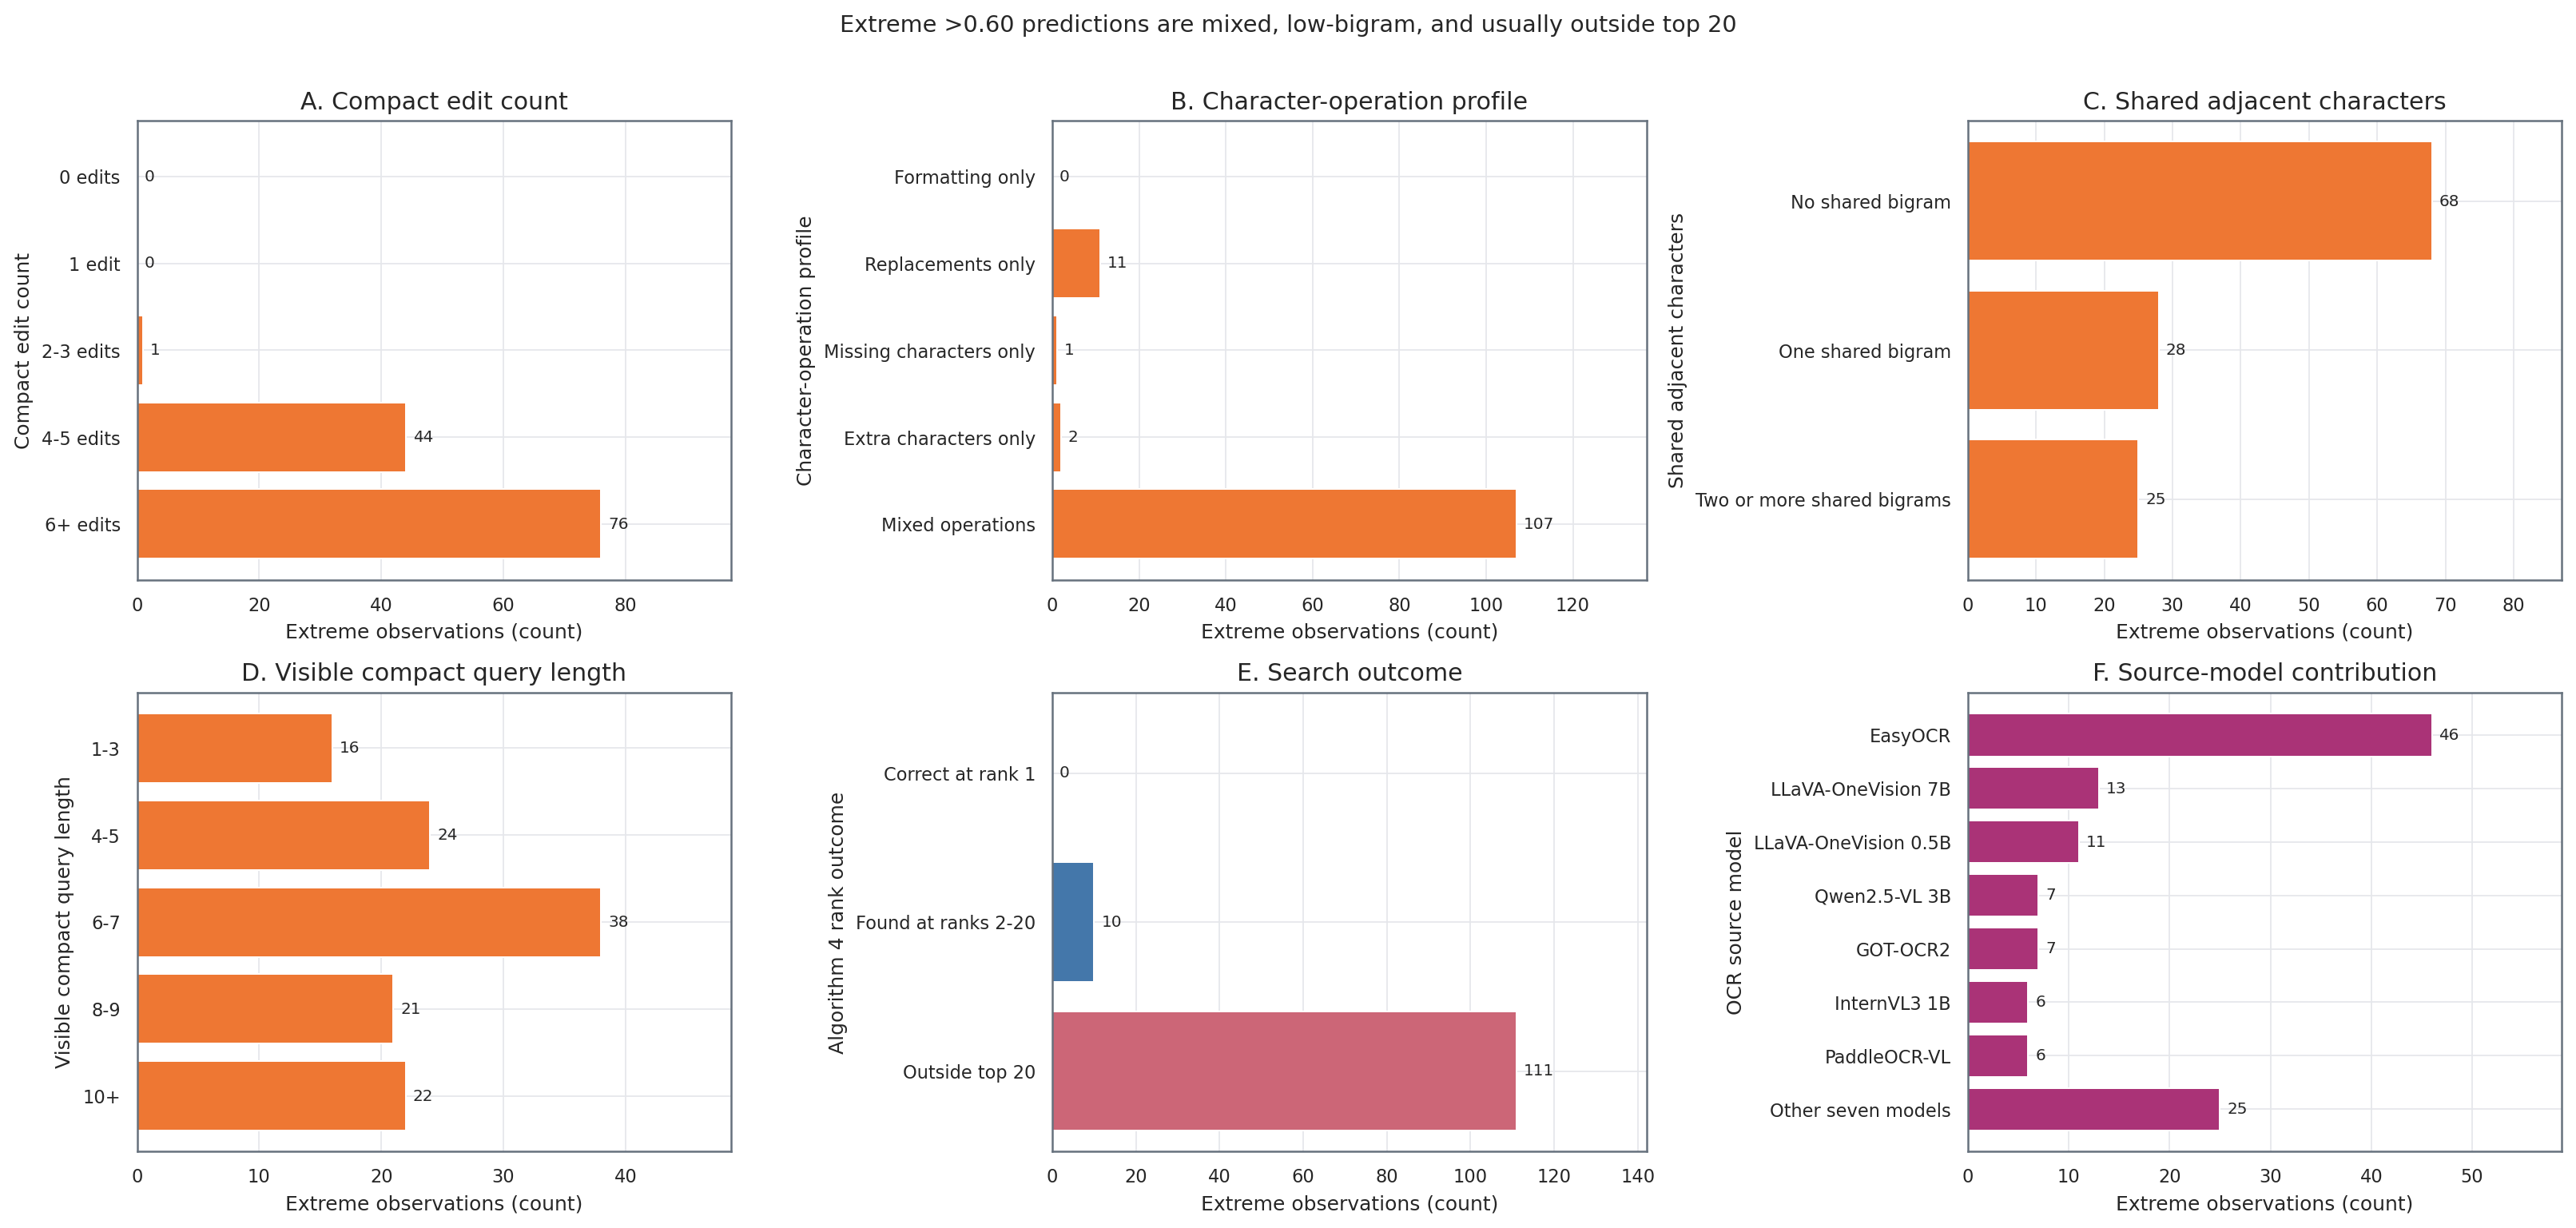
\includegraphics[width=0.90\linewidth,keepaspectratio]{06_extreme_cohort_profile.png}
\caption{All panels count the same 121 extreme observations. Panels A--D show
edit count, operation type, shared bigrams, and query length; Panel E shows
search outcome; Panel F shows case contribution, not OCR-model accuracy.}
\label{fig:extreme-cohort}
\end{figure}

\begin{minipage}{\linewidth}
\textbf{Figure 6 insights}
\begin{enumerate}
  \item The broad label hides the useful split: 107 rows are mixed-operation,
        11 replacement-only, two extra-only, and one missing-only.
  \item Bigram loss predicts failure: none of the 68 zero-bigram rows reach the
        top 20, while 8 of 25 rows with at least two shared bigrams do (32.00\%).
  \item Algorithm 4 has 0 rank-1 successes and 10 top-20 successes. After
        deduplication, Hit@20 is 9 of 113, or 7.96\%.
\end{enumerate}
\end{minipage}

\subsection{Which Extreme Rows Remain Recoverable?}

\begin{minipage}[t]{0.49\linewidth}
\textbf{Recovery by retained evidence}\par\smallskip
\small
\centering
\begin{tabular}{@{}llrrr@{}}
\toprule
\textbf{Slice} & \textbf{Group} & \textbf{Rows} & \textbf{Found} & \textbf{Hit@20} \\
\midrule
Compact edits & 2--3 & 1 & 0 & 0.00\% \\
 & 4--5 & 44 & 7 & 15.91\% \\
 & 6+ & 76 & 3 & 3.95\% \\
\addlinespace
Shared bigrams & None & 68 & 0 & 0.00\% \\
 & One & 28 & 2 & 7.14\% \\
 & Two or more & 25 & 8 & 32.00\% \\
\addlinespace
Query length & 1--3 & 16 & 1 & 6.25\% \\
 & 4--5 & 24 & 0 & 0.00\% \\
 & 6--7 & 38 & 2 & 5.26\% \\
 & 8--9 & 21 & 0 & 0.00\% \\
 & 10+ & 22 & 7 & 31.82\% \\
\bottomrule
\end{tabular}
\par\smallskip
\raggedright
Two or more shared bigrams are the clearest survival signal. Query length alone
is not monotonic and must not be used as a confidence rule.
\end{minipage}
\hfill
\begin{minipage}[t]{0.47\linewidth}
\textbf{All retrieval systems on 113 unique extreme pairs}\par\smallskip
\small
\centering
\begin{tabular}{@{}lrr@{}}
\toprule
\textbf{System} & \textbf{Found by rank 20} & \textbf{Hit@20} \\
\midrule
Jaro-Winkler & \textbf{14} & \textbf{12.3894\%} \\
Algorithm 4 & 9 & 7.9646\% \\
Character 3-gram TF-IDF & 5 & 4.4248\% \\
RapidFuzz token ratio & 4 & 3.5398\% \\
Levenshtein & 3 & 2.6549\% \\
Algorithm 3 & 3 & 2.6549\% \\
Algorithm 2 & 2 & 1.7699\% \\
Exact or prefix match & 1 & 0.8850\% \\
Phonetic baseline & 0 & 0.0000\% \\
Algorithm 1 & 0 & 0.0000\% \\
\bottomrule
\end{tabular}
\par\smallskip
\raggedright
Every system has 0\% Hit@1. Algorithm 4 and Jaro-Winkler share six top-20
successes; Algorithm 4 alone finds three and Jaro-Winkler alone finds eight.
Their 17-of-113 union is an oracle upper bound, not a deployed score.
\end{minipage}

\subsection{Concrete Extreme-Distance Rows}

\begin{center}
\centering
\small
\begin{tabularx}{\linewidth}{@{}L{0.16\linewidth}L{0.23\linewidth}L{0.18\linewidth}Y@{}}
\toprule
\textbf{OCR input $\rightarrow$ target} & \textbf{Why it exceeds 60\%} &
\textbf{Algorithm 4 result} & \textbf{What the row teaches} \\
\midrule
\code{PNO}$\rightarrow$\code{RIVO} & Mixed: one missing and two replacements; $d=3$, $r=0.75$, zero bigrams. & \code{PONO} first; target outside top 20. & Three edits are extreme because the target has only four characters. A generic first-letter rule cannot recover the lost evidence. \\
\code{RIV}$\rightarrow$\code{RIVOTRIL} & Missing only: five missing characters; $d=5$, $r=0.625$, two bigrams. & \code{RIVO} first; target rank 10. & The visible prefix supports two real families. Show both and ask whether unreadable characters follow. \\
\code{LACTULOSE}$\rightarrow$\code{LACTO} & Extra only: four extra characters; $d=4$, $r=0.80$, three bigrams. & \code{LACTULOSE HEK} first; target outside top 20. & The continuation supports another family or variant more strongly. Audit the crop and label instead of forcing \code{LACTO}. \\
\code{MYUBKL}$\rightarrow$\code{MYOLAX} & Replacements only: four replacements; $d=4$, $r=0.667$, one bigram. & \code{MYONIL} first; target rank 11. & One adjacent pair preserves enough evidence for retrieval, but not for a safe first choice. \\
\code{KETOCONAZOLE}$\rightarrow$\code{KETOROLAC} & Mixed: three extra and three replacements; $d=6$, $r=0.667$, four bigrams. & \code{BUTOCONAZOLE} first; target rank 18. & The shared \code{KETO} structure keeps the target in the list, while another complete name remains lexically stronger. \\
\code{HOAVACH}$\rightarrow$\code{AMIKACIN} & Mixed: one missing and five replacements; $d=6$, $r=0.75$, one bigram. & \code{HYABAK} first; target outside top 20. & Almost all local target structure is gone, so a small ranking bonus cannot repair candidate generation. \\
\code{H}$\rightarrow$\code{RIVO} & Mixed: three missing and one replacement; $d=4$, $r=1.00$, zero bigrams. & No candidates; target outside top 20. & One visible character cannot identify a medicine family. The interface must request more image or user evidence. \\
\bottomrule
\end{tabularx}
\par\smallskip
\begin{minipage}{0.94\linewidth}
\small\textit{Representative source rows for each important extreme-distance
shape. ``Missing'' means characters must be inserted into the OCR output;
``extra'' means OCR characters must be deleted to reach the verified target.}
\end{minipage}
\end{center}

\textbf{Engineering decisions}
\begin{enumerate}
  \item Do not present a confident family for this cohort; no tested system gets
        one of the 113 unique pairs correct at rank 1.
  \item Test Jaro-Winkler as a secondary candidate generator only for bounded
        rows with retained bigrams. Preserve Algorithm 4's clarification gate.
  \item For zero-bigram or very short inputs, request unreadable-position or
        additional-image evidence instead of adding another lexical weight.
  \item Audit repeated and real-name-like outputs before tuning. The pair
        \code{ARDANCE}$\rightarrow$\code{RIVO} appears seven times, so repeated
        model observations must not become seven independent training rules.
\end{enumerate}

\clearpage
\section{OCR Evidence and Retrieval Comparisons}

\setcounter{figure}{6}
\begin{figure}[H]
\centering
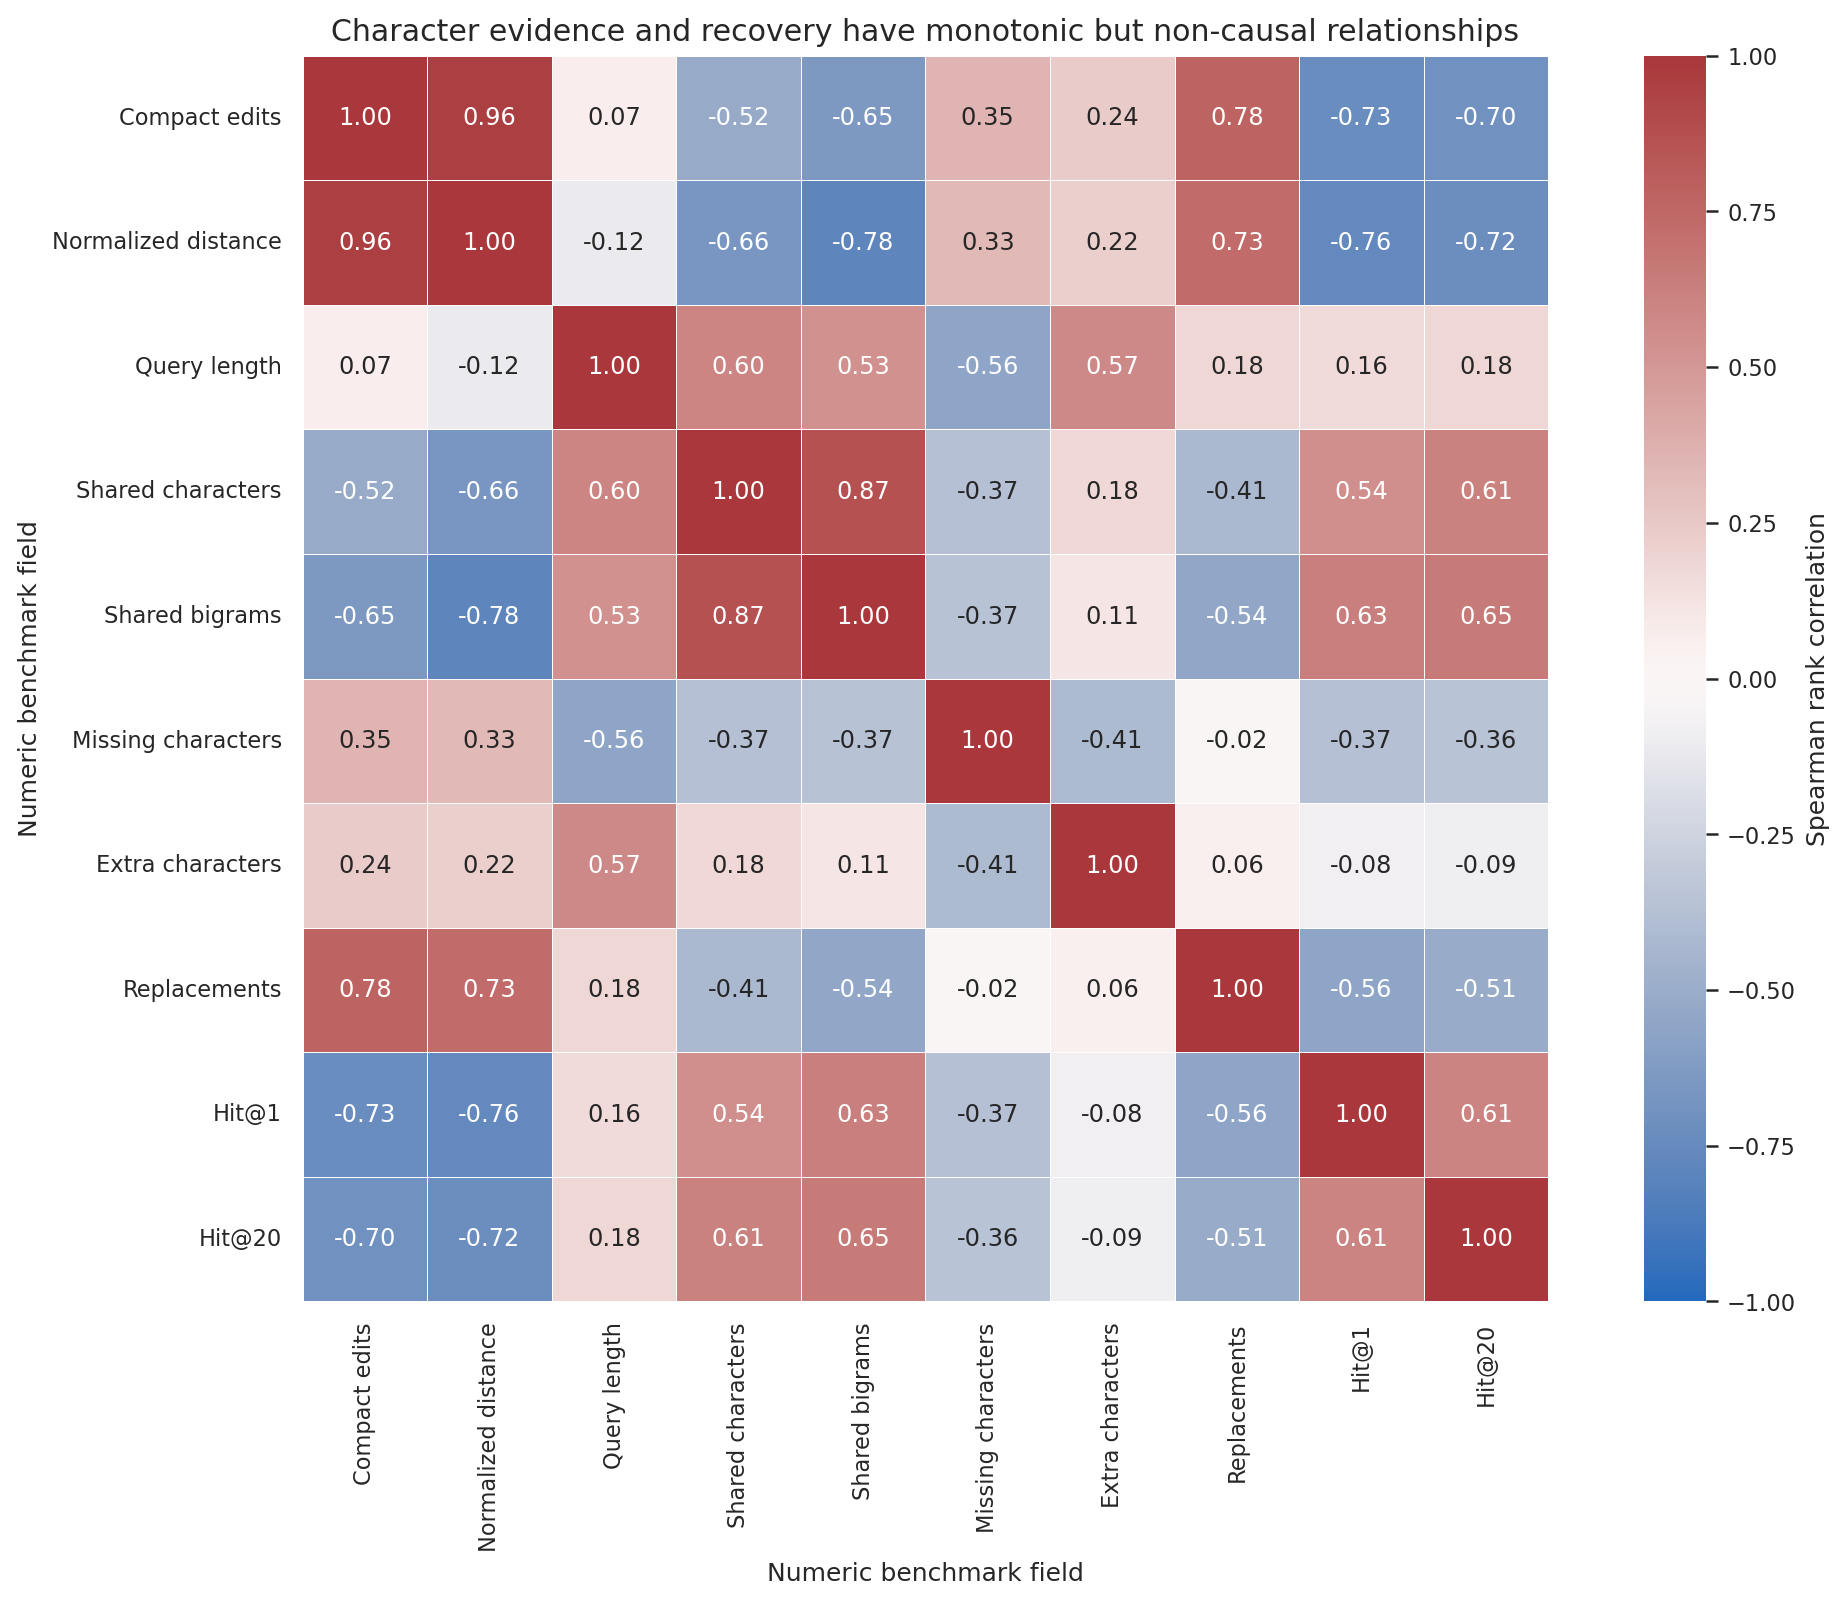
\includegraphics[width=0.96\linewidth,height=0.64\textheight,keepaspectratio]{07_ocr_correlation_matrix.png}
\caption{Each cell is a Spearman rank correlation over the same 464
primary pairs. Values near $+1$ mean two fields tend to rise together, values
near $-1$ mean one tends to fall as the other rises, and values near zero show
little monotonic relationship. Correlation describes association, not cause.}
\end{figure}

\textbf{Figure 7 insights}
\begin{enumerate}
  \item Normalized edit distance has the strongest negative relationship with
        recovery: $\rho=-0.7592$ for Hit@1 and $\rho=-0.7202$ for Hit@20.
  \item Shared bigrams have positive relationships with Hit@1
        ($\rho=0.6279$) and Hit@20 ($\rho=0.6520$), so retained adjacent-letter
        order is useful evidence.
  \item Replacement count correlates with Hit@20 at $\rho=-0.5100$, but this
        overlaps with total distance and mixed errors and is not an isolated
        causal effect.
\end{enumerate}

\clearpage
\begin{center}
\fcolorbox{LineGray}{LightYellow}{%
\begin{minipage}{0.92\linewidth}
\textbf{What is a bigram?}
After case, spaces, and punctuation are removed, a bigram is one pair of
adjacent characters. \code{MYMLAX} produces \code{MY}, \code{YM}, \code{ML},
\code{LA}, and \code{AX}. \code{MYOLAX} produces \code{MY}, \code{YO},
\code{OL}, \code{LA}, and \code{AX}. The pair therefore has three shared
bigrams: \code{MY}, \code{LA}, and \code{AX}. Shared bigrams preserve local
order; merely sharing the letters M, Y, L, A, and X does not.
\end{minipage}}
\end{center}

\begin{figure}[H]
\centering
\plot{08_distance_bigram_interaction.png}
\caption{Rows are compact edit-distance bands and columns are shared
bigram bands. The left heatmap reports Algorithm 4 Hit@20 and its denominator
inside each cell; the right heatmap repeats the case counts so small cells are
not mistaken for stable estimates.}
\end{figure}

\textbf{Figure 8 insights}
\begin{enumerate}
  \item Within four-to-five edits, Hit@20 rises from 0\% with no shared bigram
        to 24\% with one and 66\% with at least two. Bigram evidence separates
        cases even after edit distance is held in the same band.
  \item At six or more edits, two-plus shared bigrams reach only 21.4\% Hit@20.
        Bigrams help bounded corruption but cannot recover most severe rows.
\end{enumerate}

\clearpage
{\small
\setlength{\intextsep}{4pt}
\setlength{\abovecaptionskip}{3pt}
\setlength{\belowcaptionskip}{0pt}
\renewcommand{\arraystretch}{1.0}
MRR@20 gives a result at rank $r\leq20$ the value $1/r$ and gives a result
outside rank 20 the value zero. Median milliseconds measure a warm query after
index preparation. Table 12 is retained instead of Meeting 10 Figure 9 because
the table provides the exact accuracy and latency values.

\begin{table}[H]
\centering
\footnotesize
\begin{tabular}{@{}lrrrrr@{}}
\toprule
\textbf{System} & \textbf{Hit@1} & \textbf{Hit@5} & \textbf{Hit@20} &
\textbf{MRR@20} & \textbf{Median ms} \\
\midrule
Algorithm 4, family rescue & \textbf{47.6293\%} & \textbf{61.8534\%} & \textbf{71.1207\%} & \textbf{0.537476} & 14.0704 \\
Exhaustive Levenshtein & 34.2672\% & 50.8621\% & 59.2672\% & 0.416955 & 0.7039 \\
Jaro-Winkler & 32.1121\% & 55.1724\% & 67.4569\% & 0.425369 & 0.6713 \\
RapidFuzz token ratio & 31.4655\% & 48.9224\% & 59.0517\% & 0.394378 & 8.0152 \\
Algorithm 2, external fast & 25.8621\% & 43.7500\% & 51.2931\% & 0.329160 & 3.8593 \\
Algorithm 3, rank fusion & 25.6466\% & 40.9483\% & 53.0172\% & 0.326419 & 6.1017 \\
Algorithm 1, current app & 23.7069\% & 31.4655\% & 38.1466\% & 0.272602 & 0.7372 \\
Character 3-gram TF-IDF & 18.3190\% & 35.7759\% & 47.4138\% & 0.257995 & 0.5042 \\
Phonetic baseline & 6.8966\% & 16.8103\% & 23.2759\% & 0.110216 & \textbf{0.4722} \\
Exact or prefix match & 2.5862\% & 2.8017\% & 3.0172\% & 0.027155 & 0.7060 \\
\bottomrule
\end{tabular}
\caption{Exact Experiment 1 comparison over the same 464 primary pairs. Query
latency excludes preparation; Algorithm 4 prepares its combined index in
8,731.705 ms before warm queries.}
\end{table}

\textbf{Table 12 insights}
\begin{enumerate}
  \item Algorithm 4 leads every alternative at Hit@1 and Hit@20. Its Hit@1 is
        13.3621 points above exhaustive Levenshtein.
  \item Jaro-Winkler is the strongest classical Hit@20 baseline at 67.4569\%;
        Algorithm 4 adds 3.6638 points.
  \item Exact/prefix and phonetic-only retrieval are insufficient for this OCR
        error mix, with Hit@20 of 3.0172\% and 23.2759\%.
\end{enumerate}

Table 13 is retained instead of Meeting 10 Figure 10. It reports the same edit
distance comparison numerically and adds the mixed-operation column, which the
distance-only figure does not contain.

\begin{table}[H]
\centering
\footnotesize
\begin{tabular}{@{}lrrrrrr@{}}
\toprule
\textbf{System} & \textbf{Overall} & \textbf{1 edit} & \textbf{2--3} &
\textbf{4--5} & \textbf{6+} & \textbf{Mixed} \\
\midrule
Exact/prefix & 3.0\% & 6.2\% & 1.1\% & 1.1\% & 0.0\% & 0.0\% \\
Levenshtein & 59.3\% & 85.7\% & 82.8\% & 23.7\% & 0.0\% & 40.9\% \\
Jaro-Winkler & 67.5\% & \textbf{100.0\%} & 86.0\% & 32.3\% & \textbf{10.1\%} & 49.8\% \\
Character 3-gram TF-IDF & 47.4\% & 79.5\% & 57.0\% & 20.4\% & 2.9\% & 34.4\% \\
RapidFuzz token ratio & 59.1\% & 92.0\% & 80.6\% & 19.4\% & 1.4\% & 42.5\% \\
Phonetic baseline & 23.3\% & 56.2\% & 19.4\% & 6.5\% & 0.0\% & 12.1\% \\
Algorithm 1 & 38.1\% & 83.0\% & 40.9\% & 4.3\% & 0.0\% & 16.2\% \\
Algorithm 2 & 51.3\% & 96.4\% & 59.1\% & 17.2\% & 0.0\% & 31.2\% \\
Algorithm 3 & 53.0\% & 95.5\% & 62.9\% & 18.3\% & 1.4\% & 32.4\% \\
Algorithm 4 & \textbf{71.1\%} & 98.2\% & \textbf{93.5\%} & \textbf{41.9\%} & 4.3\% & \textbf{53.4\%} \\
\bottomrule
\end{tabular}
\caption{Hit@20 by compact edit count and OCR operation shape. The one-edit,
two-to-three, four-to-five, six-plus, and mixed groups contain 112, 186, 93,
69, and 247 primary pairs. Bold marks the best result in each column.}
\end{table}

\textbf{Table 13 insights}
\begin{enumerate}
  \item Algorithm 4 creates its largest advantage at bounded corruption,
        reaching 93.5\% Hit@20 for two-to-three edits and 41.9\% for four-to-five.
  \item Jaro-Winkler reaches 100\% on one-edit rows and the best six-plus result,
        10.1\%, but places the correct family first less often overall.
  \item Every method remains weak at six-plus edits. Extra image or user
        evidence is more realistic than another small ranking bonus there.
\end{enumerate}
}

\clearpage
\setcounter{figure}{10}
\begin{figure}[H]
\centering
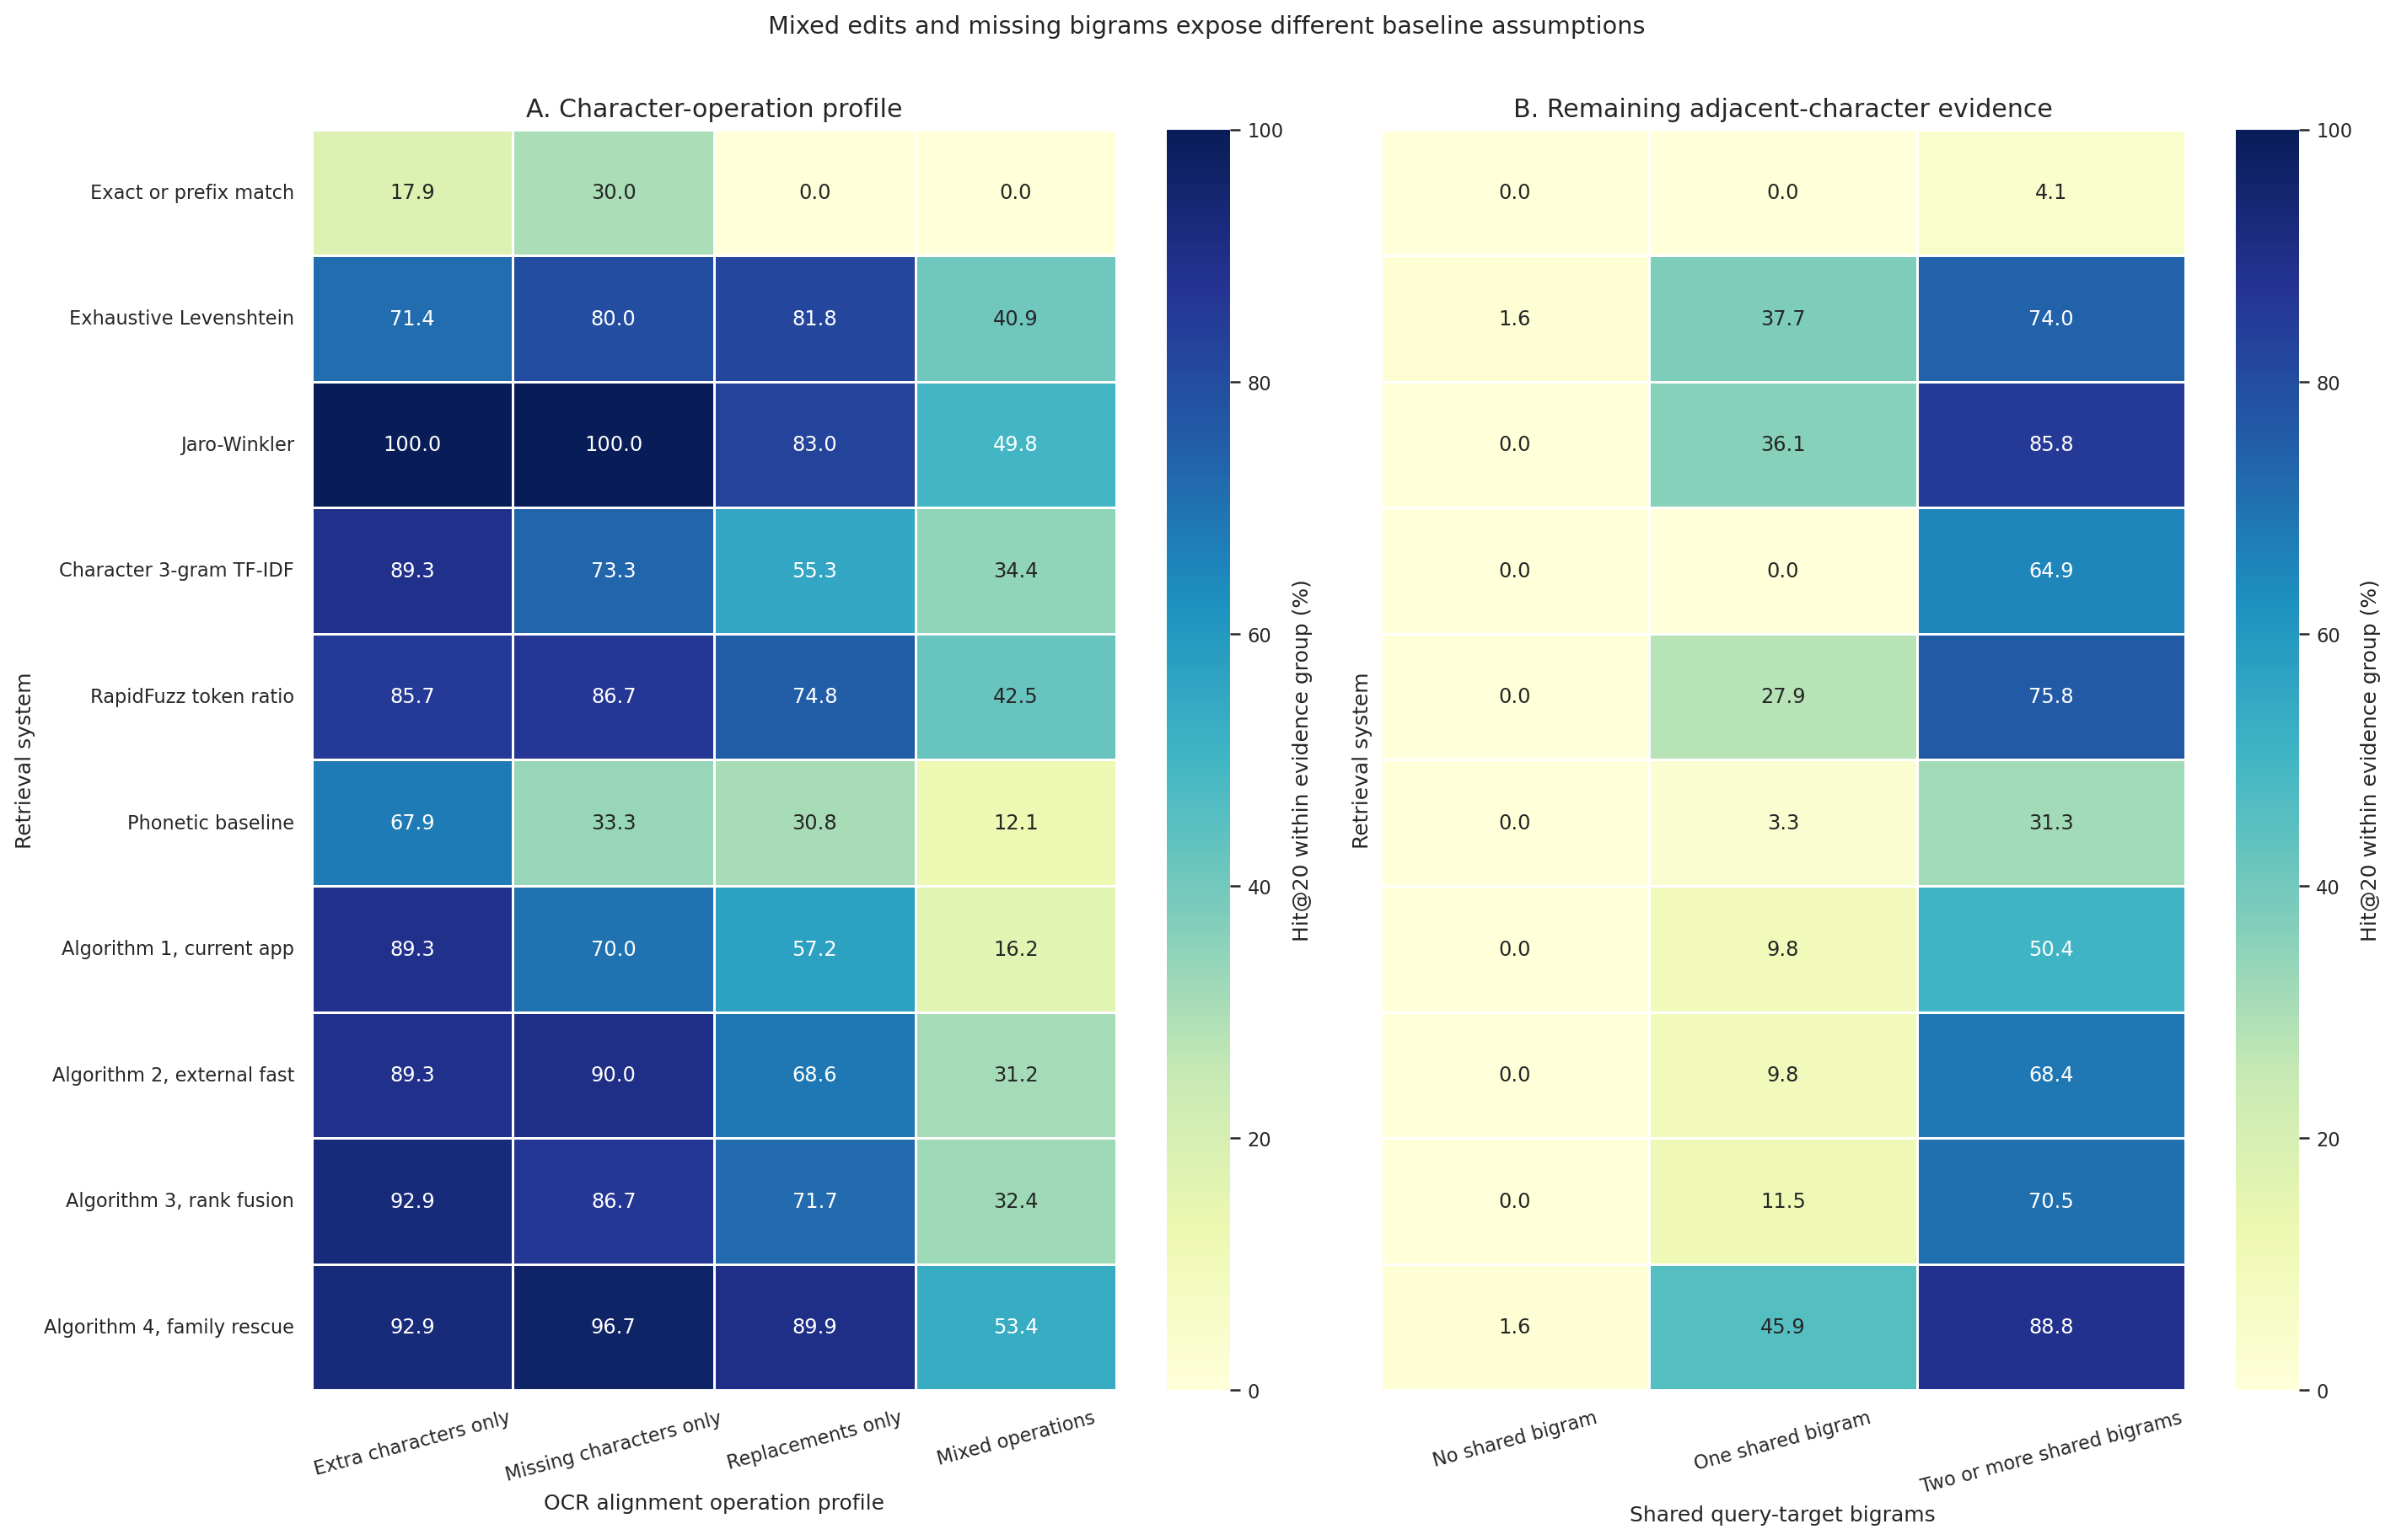
\includegraphics[width=0.96\linewidth,height=0.49\textheight,keepaspectratio]{28_retrieval_error_evidence_profiles.png}
\caption{Every cell is Hit@20 inside the named group over the same
464 pairs. Panel A separates isolated extra, missing, and replacement errors
from mixed operations. Panel B groups the number of compact query-target
bigrams, where one bigram is one shared adjacent-character pair.}
\end{figure}

{\small
\textbf{Figure 11 system-by-system insights}
\begin{enumerate}
  \item Exact/prefix handles literal fragments but almost no corruption: mixed
        and replacement-only Hit@20 are both 0\%.
  \item Levenshtein handles isolated replacements at 81.8\% but falls to 40.9\%
        on mixed operations because every edit has the same cost.
  \item Jaro-Winkler reaches 100\% on isolated additions and deletions and 49.8\%
        on mixed edits, but 0\% when no bigram remains.
  \item Character 3-gram TF-IDF reaches 64.9\% with at least two bigrams and 0\%
        with zero or one because a three-character feature cannot be formed from
        a single two-character overlap.
  \item RapidFuzz reaches 75.8\% with two-plus bigrams and 42.5\% on mixed edits,
        but token spacing can change its score.
  \item The phonetic baseline reaches 31.3\% with two-plus bigrams and 12.1\% on
        mixed edits. Sound keys are supporting evidence, not a full ranker.
  \item Algorithm 1 reaches 57.2\% on replacement-only rows but 16.2\% on mixed
        rows because its candidate expansion is conservative.
  \item Algorithm 2 raises mixed-operation Hit@20 to 31.2\% and handles missing
        characters at 90.0\%, but still needs a safety gate.
  \item Algorithm 3 reaches 32.4\% on mixed rows and 70.5\% with two-plus
        bigrams; fusion alone does not add Algorithm 4 family-rescue candidates.
  \item Algorithm 4 leads mixed rows at 53.4\% and one-bigram rows at 45.9\%,
        but zero-bigram Hit@20 is only 1.6\%. It extends bounded evidence rather
        than guessing from unrelated text.
\end{enumerate}
}

\clearpage
\begin{figure}[H]
\centering
\plot{29_retrieval_failure_composition.png}
\caption{Each horizontal bar contains only that system's top-20
misses. Segment width is the percentage of those misses in each compact edit
band; the label beside the system gives its total miss count. This figure shows
failure composition, not accuracy.}
\end{figure}

\textbf{Figure 12 insights}
\begin{enumerate}
  \item Algorithm 4 has the fewest misses, 134. Four-or-more edits create 120,
        or 89.55\%, so its remaining failures are concentrated in severe rows.
  \item Exact/prefix misses 450 pairs, including 105 one-edit and 184
        two-to-three-edit rows. It fails ordinary corruption, not only the tail.
  \item Jaro-Winkler misses 151 pairs, only 17 more than Algorithm 4, but the
        methods do not fail on exactly the same rows.
\end{enumerate}

\clearpage
\setcounter{figure}{14}
\begin{figure}[H]
\centering
\plot{12_query_latency_distributions.png}
\caption{Each horizontal box plot summarizes 464 warm-query times.
The line inside a box is the median, the box is the middle 50\%, and the
whiskers show the non-outlier range. The panels use different x-axis scales so
sub-millisecond systems remain readable beside slower systems.}
\end{figure}

\textbf{Figure 15 insights}
\begin{enumerate}
  \item Algorithm 4 has mean latency 14.8852 ms, median 14.0704 ms, and a
        measured 95th percentile of 30.1791 ms. A single average hides this tail.
  \item RapidFuzz has an 8.0152 ms median despite weaker retrieval than the
        sub-1-ms Levenshtein and Jaro-Winkler implementations. Library naming
        does not determine speed for this workload.
  \item These are warm single-process timings after index preparation, not
        concurrent production throughput.
\end{enumerate}

\clearpage
\section{Fair Versus Inclusive Synthetic Scoring}

\textbf{Inclusive} counts all 115,000 generated rows. \textbf{Fair} keeps the
same file but removes 5,026 exact-real-name collisions from single-answer
accuracy by setting \code{scored\_case=0}; 109,974 rows remain scored. The rows
are not deleted and still participate in safety and ambiguity diagnostics.

\begin{table}[H]
\centering
\small
\begin{tabularx}{\linewidth}{@{}L{0.20\linewidth}L{0.22\linewidth}L{0.22\linewidth}Y@{}}
\toprule
\textbf{Entered query} & \textbf{Generated expected family} &
\textbf{Exact real family already named} & \textbf{Why fair scoring removes it} \\
\midrule
\code{epigent} & \code{APIGENT} & \code{EPIGENT} & The literal input is already a different valid catalog medicine. \\
\code{eviton} & \code{A VITON} & \code{E VITON} & Ranking the exact entered family first is reasonable, not a search error. \\
\code{benox} & \code{BANOX} & \code{BENOX} & The mutation created another real name, so one mandatory target is unfair. \\
\bottomrule
\end{tabularx}
\caption{Examples among the 5,026 rows excluded only from fair single-answer
accuracy. They remain available for collision and safety analysis.}
\end{table}

\begin{table}[H]
\centering
\small
\setlength{\tabcolsep}{6pt}
\begin{tabular}{@{}lrrrrrr@{}}
\toprule
\textbf{Algorithm} & \textbf{Incl. H@1} & \textbf{Fair H@1} &
\textbf{Incl. H@20} & \textbf{Fair H@20} & \textbf{Fair behavior} &
\textbf{Fair unsafe} \\
\midrule
Algorithm 1 & 75.2565\% & 78.6841\% & 88.4043\% & 90.6578\% & 90.9260\% & 0.0173\% \\
Algorithm 2 & 79.3009\% & 82.9251\% & 91.8374\% & 93.9740\% & 93.3975\% & 2.8407\% \\
Algorithm 3 & 81.0348\% & 84.7373\% & 93.0948\% & 95.3389\% & 95.5799\% & \textbf{0.0000\%} \\
Algorithm 4 & \textbf{82.1165\%} & \textbf{85.8694\%} & \textbf{93.4122\%} & \textbf{95.6490\%} & \textbf{95.8845\%} & \textbf{0.0000\%} \\
\bottomrule
\end{tabular}
\caption{Inclusive uses 115,000 rows and fair uses 109,974. The same
collision rule is applied to all four algorithms; no source row is deleted.}
\end{table}

\textbf{Table 15 insights}
\begin{enumerate}
  \item Fair Hit@1 rises by 3.4275, 3.6242, 3.7025, and 3.7529 points for
        Algorithms 1--4 because exact-name collisions no longer count as
        single-answer mistakes.
  \item Algorithm order is unchanged at both cutoffs: Algorithm 4 remains
        first, followed by Algorithms 3, 2, and 1.
  \item Algorithm 2 still has 2.8407\% unsafe confident first results after
        collision removal, so collisions explain only part of its safety issue.
\end{enumerate}



\end{document}
